\documentclass[10pt,border=6pt]{standalone}

\usepackage{amsmath}
\usepackage{amssymb}
\usepackage{tikz}
\usetikzlibrary{arrows.meta,positioning}

\hyphenpenalty=10000
\exhyphenpenalty=10000

\begin{document}
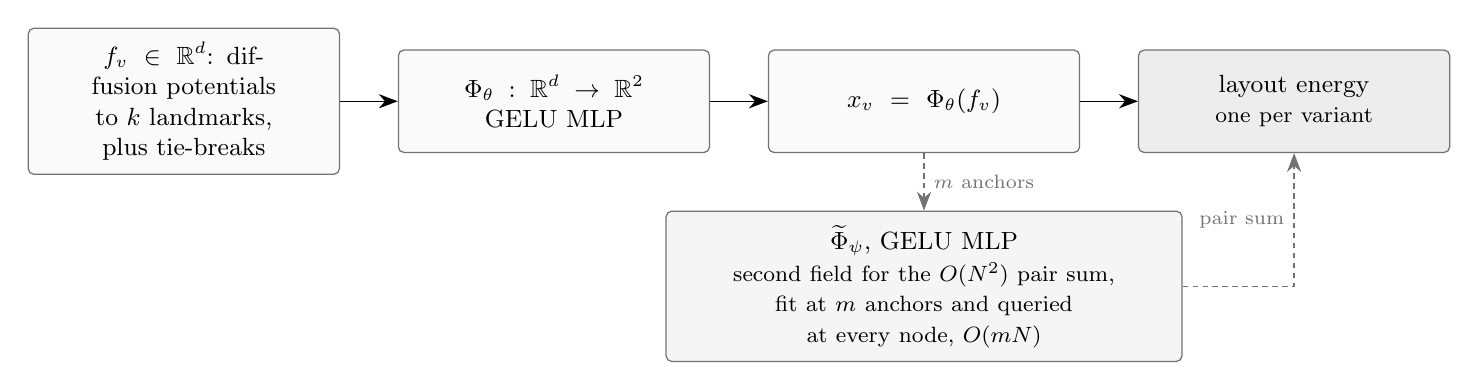
\begin{tikzpicture}[
  font=\small,
  box/.style   ={draw=black!55, rounded corners=2pt, align=center,
                 inner sep=5pt, line width=0.45pt, fill=black!2},
  feat/.style  ={box, text width=36mm, minimum height=13mm},
  net/.style   ={box, text width=36mm, minimum height=13mm},
  coord/.style ={box, text width=36mm, minimum height=13mm},
  energy/.style={box, text width=36mm, minimum height=13mm, fill=black!7},
  far/.style   ={box, text width=62mm, fill=black!4},
  arr/.style   ={-{Stealth[length=2.4mm]}, line width=0.55pt},
  darr/.style  ={-{Stealth[length=2.4mm]}, dashed, dash pattern=on 2pt off 1.6pt,
                 line width=0.5pt, black!55},
  lbl/.style   ={font=\scriptsize, black!55},
]

\def\xf{0}
\def\xn{4.7}
\def\xc{9.4}
\def\xe{14.1}

\node[feat]   (f) at (\xf,0) {$f_v\in\mathbb{R}^d$: diffusion potentials\\to $k$ landmarks, plus tie-breaks};
\node[net]    (m) at (\xn,0) {$\Phi_\theta:\mathbb{R}^{d}\rightarrow\mathbb{R}^2$\\GELU MLP};
\node[coord]  (p) at (\xc,0) {$x_v=\Phi_\theta(f_v)$};
\node[energy] (e) at (\xe,0) {layout energy\\{\footnotesize one per variant}};

\draw[arr] (f) -- (m);   \draw[arr] (m) -- (p);   \draw[arr] (p) -- (e);

\node[far] (g) at (\xc,-2.35) {%
  $\widetilde\Phi_\psi$, GELU MLP\\[2pt]
  {\footnotesize second field for the $O(N^2)$ pair sum,\\
   fit at $m$ anchors and queried at every node, $O(mN)$}};

\draw[darr] (p) -- node[lbl,right,pos=0.5] {$m$ anchors} (p|-g.north);
\draw[darr] (g) -- (\xe,-2.35) -- node[lbl,left,pos=0.5] {pair sum} (e.south);


\end{tikzpicture}
\end{document}
